\chapter{\'Etat de l'Art et \'Etude Comparative}

\section*{Introduction}
\par Ce deuxi\`eme chapitre \'etablit les fondements th\'eoriques, m\'ethodologiques et technologiques n\'ecessaires \`a la conception de notre plateforme. Nous commen\c{c}ons par exposer les principes fondamentaux de la cybers\'ecurit\'e et analysons les dix risques majeurs du r\'ef\'erentiel OWASP Top 10. Nous d\'eveloppons ensuite les concepts cl\'es de la gestion continue de la surface d'attaque (\textit{Attack Surface Management} -- ASM) et pr\'esentons en d\'etail les m\'ecanismes internes des outils de reconnaissance de r\'ef\'erence. Par la suite, nous approfondissons le paradigme DevSecOps, la s\'ecurit\'e de la cha\^ine logicielle, l'apport de l'intelligence artificielle locale contrainte et les architectures microservices \'ev\'enementielles. Enfin, nous menons une \'etude comparative syst\'ematique qui justifie rationnellement chaque choix technologique au regard des exigences du projet.

\section{Fondements de la Cybers\'ecurit\'e}
\subsection{D\'efinition et Enjeux Contemporains}
\par La cybers\'ecurit\'e regroupe l'ensemble des technologies, processus et mesures de contr\^ole con\c{c}us pour prot\'eger les syst\`emes informatiques, les r\'eseaux, les programmes et les donn\'ees contre les cyberattaques. Selon l'Union Internationale des T\'el\'ecommunications (UIT)~\cite{itu}, l'expansion du num\'erique s'accompagne d'une professionnalisation accrue des menaces. Les organisations modernes, dont les activit\'es reposent sur des infrastructures interconnect\'ees et expos\'ees sur Internet, sont r\'eguli\`erement la cible d'attaques visant le vol de propri\'et\'e intellectuelle, l'interruption d'activit\'e ou l'extorsion de fonds. Cybersecurity Ventures~\cite{cyberventures} estime le co\^ut annuel mondial de la cybercriminalit\'e \`a plusieurs milliers de milliards de dollars, soulignant l'obligation pour les entreprises de d\'eployer des approches d'audit continues et proactives.

\subsection{Piliers Fondamentaux de la S\'ecurit\'e}
\par La posture de s\'ecurit\'e d'un syst\`eme d'information repose traditionnellement sur la triade \textbf{CIA} (Confidentialit\'e, Int\'egrit\'e, Disponibilit\'e) et ses principes directeurs associ\'es :
\begin{itemize}
    \item \textbf{Confidentialit\'e :} Garantie que les informations ne sont divulgu\'ees qu'aux personnes, processus ou syst\`emes d\^ument autoris\'es. Sa mise en \oe uvre repose sur des m\'ecanismes de chiffrement fort en transit (TLS 1.3) et au repos (AES-256), associ\'es \`a un contr\^ole d'acc\`es strict.
    \item \textbf{Int\'egrit\'e :} Pr\'eservation de l'exactitude, de la compl\'etude et de la non-alt\'eration des donn\'ees tout au long de leur cycle de vie, garantie par des signatures num\'eriques et des fonctions de hachage cryptographique (SHA-256).
    \item \textbf{Disponibilit\'e :} Maintien de l'accessibilit\'e op\'erationnelle et de la continuit\'e de service pour les utilisateurs l\'egitimes face aux pannes mat\'erielles, aux congestions r\'eseau ou aux attaques volum\'etriques.
    \item \textbf{Authentification et Autorisation :} Processus \`a deux facteurs consistant d'abord \`a prouver formellement l'identit\'e revendiqu\'ee (\textit{Authentification}), puis \`a valider les privil\`eges attribu\'es selon le principe du moindre privil\`ege (\textit{Autorisation}).
    \item \textbf{Tra\c{c}abilit\'e et Non-r\'epudiation :} Capacit\'e d'attribuer sans \'equivoque toute action ou transaction \`a une entit\'e donn\'ee, emp\^echant la contestation ult\'erieure gr\^ace \`a des journaux d'audit immuables et horodat\'es.
\end{itemize}

\section{Le R\'ef\'erentiel OWASP Top 10}
\par L'\textit{Open Worldwide Application Security Project} (OWASP)~\cite{owasp2021} est une autorit\'e de r\'ef\'erence internationale en s\'ecurit\'e applicative. Son classement d\'ecennal \textbf{OWASP Top 10} synth\'etise les risques de s\'ecurit\'e les plus r\'epandus et les plus critiques affectant les architectures web :
\begin{itemize}
    \item \textbf{A01:2021 -- Rupture du Contr\^ole d'Acc\`es (Broken Access Control) :} D\'efaillances dans l'application des restrictions d'acc\`es permettant \`a des utilisateurs non privil\'egi\'es d'acc\'eder \`a des ressources prot\'eg\'ees ou d'alt\'erer des enregistrements appartenant \`a des tiers (failles IDOR, contournement de contr\^ole RBAC).
    \item \textbf{A02:2021 -- D\'efaillances Cryptographiques (Cryptographic Failures) :} Utilisation d'algorithmes obsol\`etes (MD5, SHA1), absence de chiffrement des donn\'ees sensibles ou transmission non s\'ecuris\'ee en clair sur le r\'eseau.
    \item \textbf{A03:2021 -- Injections (Injection) :} D\'efaut de neutralisation des donn\'ees fournies par l'utilisateur, permettant d'ex\'ecuter des instructions arbitraires dans un interpr\'eteur (injections SQL, injections de commandes syst\`eme, Cross-Site Scripting).
    \item \textbf{A04:2021 -- Conception Non S\'ecuris\'ee (Insecure Design) :} Faiblesses architecturales r\'esultant de l'absence de mod\'elisation des menaces et d'application des principes de conception s\'ecuris\'ee d\`es l'amont du projet.
    \item \textbf{A05:2021 -- Mauvaise Configuration de S\'ecurit\'e (Security Misconfiguration) :} Services ou ports superflus activ\'es, messages d'erreur verbeux r\'ev\'elant des traces de pile, identifiants par d\'efaut non modifi\'es ou absence d'en-t\^etes de s\'ecurit\'e (HSTS, CSP).
    \item \textbf{A06:2021 -- Composants Vuln\'erables et Obsol\`etes :} Utilisation de biblioth\`eques, d\'ependances logicielles ou modules tiers contenant des failles document\'ees dans les bases de vuln\'erabilit\'es publiques (CVEs).
    \item \textbf{A07:2021 -- D\'efaillances d'Identification et d'Authentification :} Vuln\'erabilit\'es facilitant le bourrage d'identifiants (\textit{credential stuffing}), l'\'enum\'eration de comptes ou le d\'etournement de session.
    \item \textbf{A08:2021 -- Manque d'Int\'egrit\'e des Donn\'ees et du Logiciel :} Risques li\'es \`a la d\'es\'erialisation d'objets non s\'ecuris\'ee ou \`a l'inclusion de composants logiciels non v\'erifi\'es dans les cha\^ines CI/CD.
    \item \textbf{A09:2021 -- D\'efaillances de Journalisation et de Surveillance :} Absence ou insuffisance de journaux d'audit, retardant la d\'etection des intrusions et rendant impossibles les investigations m\'edico-l\'egales.
    \item \textbf{A10:2021 -- Falsification de Requ\^ete C\^ot\'e Serveur (SSRF) :} Vuln\'erabilit\'e permettant \`a un attaquant d'inciter l'application c\^ot\'e serveur \`a \'emettre une requ\^ete HTTP/TCP vers une ressource interne non expos\'ee.
\end{itemize}

\par La figure~\ref{fig:owasp_heat} positionne ces dix cat\'egories de risques selon leur niveau d'exploitabilit\'e et de d\'etectabilit\'e.

\begin{figure}[H]
\centering
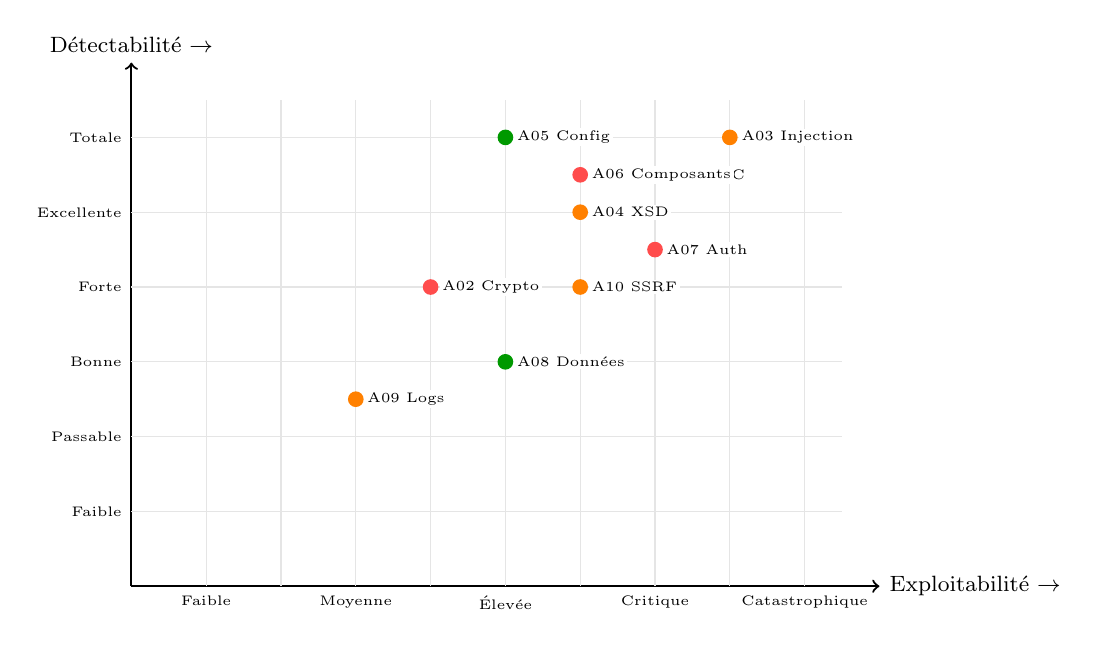
\begin{tikzpicture}[scale=0.95]
\draw[->, thick] (0,0) -- (10,0) node[right, font=\footnotesize]{Exploitabilit\'e $\rightarrow$};
\draw[->, thick] (0,0) -- (0,7) node[above, font=\footnotesize]{D\'etectabilit\'e $\rightarrow$};
\foreach \x in {1,2,3,4,5,6,7,8,9} \draw[gray!20] (\x,0) -- (\x,6.5);
\foreach \y in {1,2,3,4,5,6} \draw[gray!20] (0,\y) -- (9.5,\y);
\foreach \x/\l in {1/Faible,3/Moyenne,5/\'Elev\'ee,7/Critique,9/Catastrophique}
    \node[font=\tiny, below] at (\x,0) {\l};
\foreach \y/\l in {1/Faible,2/Passable,3/Bonne,4/Forte,5/Excellente,6/Totale}
    \node[font=\tiny, left] at (0,\y) {\l};
\node[circle, fill=red!70, inner sep=2pt, label={[font=\tiny, fill=white, inner sep=1pt]right:A01 BAC}] at (7,5.5) {};
\node[circle, fill=red!70, inner sep=2pt, label={[font=\tiny, fill=white, inner sep=1pt]right:A02 Crypto}] at (4,4) {};
\node[circle, fill=orange, inner sep=2pt, label={[font=\tiny, fill=white, inner sep=1pt]right:A03 Injection}] at (8,6) {};
\node[circle, fill=orange, inner sep=2pt, label={[font=\tiny, fill=white, inner sep=1pt]right:A04 XSD}] at (6,5) {};
\node[circle, fill=green!60!black, inner sep=2pt, label={[font=\tiny, fill=white, inner sep=1pt]right:A05 Config}] at (5,6) {};
\node[circle, fill=red!70, inner sep=2pt, label={[font=\tiny, fill=white, inner sep=1pt]right:A06 Composants}] at (6,5.5) {};
\node[circle, fill=red!70, inner sep=2pt, label={[font=\tiny, fill=white, inner sep=1pt]right:A07 Auth}] at (7,4.5) {};
\node[circle, fill=green!60!black, inner sep=2pt, label={[font=\tiny, fill=white, inner sep=1pt]right:A08 Donn\'ees}] at (5,3) {};
\node[circle, fill=orange, inner sep=2pt, label={[font=\tiny, fill=white, inner sep=1pt]right:A09 Logs}] at (3,2.5) {};
\node[circle, fill=orange, inner sep=2pt, label={[font=\tiny, fill=white, inner sep=1pt]right:A10 SSRF}] at (6,4) {};
\end{tikzpicture}
\caption{Matrice des Risques OWASP Top 10 (2021) -- Exploitabilit\'e vs D\'etectabilit\'e}
\label{fig:owasp_heat}
\end{figure}

\section{Gestion Continue de la Surface d'Attaque (ASM)}
\subsection{D\'efinition et Principes}
\par La surface d'attaque d'une organisation repr\'esente l'ensemble cumul\'e des points d'entr\'ee et vecteurs d'exposition par lesquels un attaquant potentiel peut tenter d'infiltrer un r\'eseau, de corrompre un syst\`eme ou d'exfiltrer des donn\'ees. L'\textit{Attack Surface Management} (ASM) est la discipline d'ing\'enierie consistant \`a identifier, cartographier, analyser et r\'eduire en continu cette surface d'exposition num\'erique externe.

\subsection{Cycle de Vie du Processus ASM}
\par Une d\'emarche ASM mature s'organise selon un cycle it\'eratif structur\'e en six phases interd\'ependantes, illustr\'e sur la figure~\ref{fig:asm_flow} :
\begin{enumerate}
    \item \textbf{D\'ecouverte (Discovery) :} Recherche et d\'etection exhaustive de tous les actifs expos\'es sur Internet associ\'es \`a l'organisation (domaines, sous-domaines, plages IP, services Cloud, certificats).
    \item \textbf{Inventaire (Inventory) :} Structuration et centralisation des donn\'ees d'actifs au sein d'un r\'ef\'erentiel d'inventaire unifi\'e.
    \item \textbf{Classification (Classification) :} \'Evaluation de la nature des actifs, de leur niveau d'exposition et de leur criticit\'e m\'etier.
    \item \textbf{Audit et Analyse (Assessment) :} Ex\'ecution de scans techniques cibl\'es pour d\'etecter les vuln\'erabilit\'es, faiblesses applicatives et d\'efauts de configuration.
    \item \textbf{Priorisation (Prioritization) :} \'Evaluation du rayon d'impact (\textit{blast radius}) et corr\'elation relationnelle pour hi\'erarchiser les alertes en fonction de la menace r\'eelle.
    \item \textbf{Rem\'ediation (Remediation) :} D\'eploiement de correctifs logiciels, durcissement des r\`egles de filtrage et validation post-rem\'ediation.
\end{enumerate}

\begin{figure}[H]
    \centering
    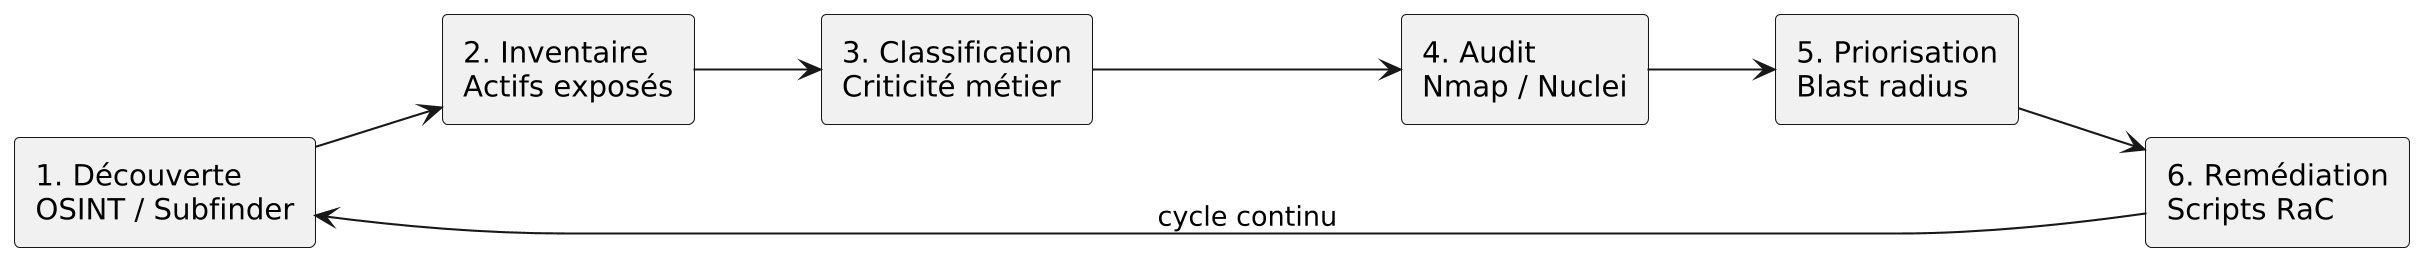
\includegraphics[width=0.95\textwidth]{img/fig_2_2_asm.png}
    \caption{Cycle de Vie du Processus d'Attack Surface Management (ASM)}
    \label{fig:asm_flow}
\end{figure}

\section{Reconnaissance et Outils d'Audit de S\'ecurit\'e}
\subsection{R\^ole et Typologie de la Reconnaissance}
\par La reconnaissance constitue la premi\`ere phase incontournable de tout audit technique de s\'ecurit\'e. Elle se d\'ecompose en deux grandes modalit\'es :
\begin{itemize}
    \item \textbf{Reconnaissance Passive (OSINT) :} Collecte d'informations sans interaction r\'eseau directe avec l'infrastructure de la cible (interrogation des registres WHOIS, des serveurs DNS publics, des registres de transparence de certificats \texttt{crt.sh}). Elle garantit une discr\'etion op\'erationnelle totale.
    \item \textbf{Reconnaissance Active :} \'Emission de paquets r\'eseau et de requ\^etes applicatives directement vers les h\^otes cibles (balayage de ports SYN, requ\^etes HTTP/HTTPS, \'enum\'eration de r\'epertoires). Elle fournit une cartographie technique exacte des services et versions expos\'es.
\end{itemize}

\subsection{Outils d'Audit Int\'egr\'es dans la Plateforme}
\par Notre plateforme int\`egre cinq outils de reconnaissance et d'audit de s\'ecurit\'e de r\'ef\'erence, encapsul\'es au sein de conteneurs isol\'es :

\begin{itemize}
    \item \textbf{\color{blue!80!black}[\,Nmap\,] -- Network Mapper~\cite{nmap} :} Outil d'exploration r\'eseau mondialement reconnu. Il utilise l'\'emission de paquets TCP SYN bruts (\textit{SYN stealth scan}) pour d\'eterminer l'\'etat des ports, identifie les banni\`eres applicatives et d\'etecte les syst\`emes d'exploitation via l'analyse de signatures TCP/IP. Son moteur NSE (\textit{Nmap Scripting Engine}) permet d'ex\'ecuter des scripts Lua pour \'evaluer des vuln\'erabilit\'es connues.
    \item \textbf{\color{purple!80!black}[\,Nuclei\,] -- Vulnerability Scanner~\cite{nuclei} :} Moteur d'\'evaluation de vuln\'erabilit\'es pilot\'e par des mod\`eles d\'eclaratifs YAML communautaires. Con\c{c}u en langage Go, il excelle dans la d\'etection rapide de failles web complexes (CVEs r\'ecentes, faiblesses d'authentification, fuites de donn\'ees d'infrastructure) en envoyant des requ\^etes cibl\'ees avec un taux de faux positifs inf\'erieur aux scanners g\'en\'eriques.
    \item \textbf{\color{cyan!80!black}[\,Gobuster\,] -- Content \& DNS Enumeration~\cite{gobuster} :} Outil d'\'enum\'eration brute rapide d\'evelopp\'e en Go exploitant des routines concurrentes. Il permet d'identifier les chemins, r\'epertoires cach\'es, fichiers sensibles d'environnement (\texttt{.env}, \texttt{.git}, sauvegardes \texttt{.bak}) et sous-domaines par confrontation \`a des dictionnaires volumineux (\textit{SecLists}).
    \item \textbf{\color{green!60!black}[\,Subfinder\,] -- Passive OSINT Subdomains~\cite{subfinder} :} Outil d'\'enum\'eration passive de sous-domaines. Il agr\`ege les donn\'ees issues de dizaines de sources passives ouvertes sans jamais contacter directement la cible, assurant la d\'ecouverte exhaustive des p\'erim\`etres oubli\'es.
    \item \textbf{\color{orange!80!black}[\,WPScan\,] -- WordPress Vulnerability Scanner~\cite{wpscan} :} Scanner sp\'ecialis\'e dans l'audit des syst\`emes WordPress. Il analyse le code source HTML, les en-t\^etes HTTP et les r\'epertoires standards pour recenser les th\`emes et extensions obsol\`etes r\'epertori\'es dans la base de donn\'ees WPScan Vulnerability Database.
\end{itemize}

\section{DevSecOps et S\'ecurit\'e de la Cha\^ine Logicielle}
\subsection{Origine et Philosophie Shift-Left}
\par Le mod\`ele traditionnel de d\'eveloppement logiciel r\'eservait les contr\^oles de s\'ecurit\'e \`a la fin du cycle de livraison, juste avant le passage en production. Cette approche tardive engendrait des goulots d'\'etranglement op\'erationnels majeurs : la correction d'une faille architecturale ou d'une d\'ependance vuln\'erable d\'ecouverte tardivement entra\^inant des co\^uts prohibitifs et des retards de d\'eploiement importants.
\par Le paradigme \textbf{DevSecOps}~\cite{devsecops} propose de fusionner le d\'eveloppement (\textit{Dev}), la s\'ecurit\'e (\textit{Sec}) et les op\'erations (\textit{Ops}) en int\'egrant des contr\^oles automatis\'es \`a chaque \'etape du cycle de vie logiciel, comme l'illustre la figure~\ref{fig:devsecops_cycle}. Cette philosophie, qualifi\'ee de \textbf{\textit{Shift-Left Security}}, consiste \`a d\'eplacer les v\'erifications de s\'ecurit\'e le plus t\^ot possible dans la cha\^ine de fabrication logicielle, permettant aux d\'eveloppeurs d'identifier et de corriger les vuln\'erabilit\'es d\`es la phase d'\'ecriture du code source.

\begin{figure}[H]
\centering
\begin{tikzpicture}[
    node distance=5mm and 6mm,
    stage/.style={draw, rounded corners=3pt, fill=blue!8, draw=blue!50, thick, minimum width=24mm, minimum height=10mm, align=center, font=\tiny\bfseries},
    secgate/.style={draw, rounded corners=3pt, fill=red!10, draw=red!60, thick, minimum width=24mm, minimum height=8mm, align=center, font=\tiny},
    arrow/.style={-{Stealth[length=2mm]}, thick, draw=blue!70}
]
\node[stage] (plan) {1. Planifier\\\& Coder};
\node[stage, right=of plan] (build) {2. Construire\\\& Tester};
\node[stage, right=of build] (scan) {3. Scanner\\\& Valider};
\node[stage, right=of scan] (sign) {4. Signer\\\& Publier};
\node[stage, right=of sign] (deploy) {5. D\'eployer\\en Prod};

\node[secgate, below=4mm of plan] (g1) {IDE Linting\\Pre-commit};
\node[secgate, below=4mm of build] (g2) {SAST (Psalm/Bandit)\\SCA D\'ependances};
\node[secgate, below=4mm of scan] (g3) {SBOM (Syft)\\Trivy Container};
\node[secgate, below=4mm of sign] (g4) {Cosign Signature\\Attestation OCI};
\node[secgate, below=4mm of deploy] (g5) {UFW + Nginx TLS\\Audit Logs};

\draw[arrow] (plan) -- (build);
\draw[arrow] (build) -- (scan);
\draw[arrow] (scan) -- (sign);
\draw[arrow] (sign) -- (deploy);

\draw[dashed, ->, draw=red!70] (g1) -- (plan);
\draw[dashed, ->, draw=red!70] (g2) -- (build);
\draw[dashed, ->, draw=red!70] (g3) -- (scan);
\draw[dashed, ->, draw=red!70] (g4) -- (sign);
\draw[dashed, ->, draw=red!70] (g5) -- (deploy);
\end{tikzpicture}
\caption{Cycle de Livraison DevSecOps : Int\'egration Continue des Portes de S\'ecurit\'e (Shift-Left)}
\label{fig:devsecops_cycle}
\end{figure}

\subsection{S\'ecurit\'e de la Cha\^ine d'Approvisionnement Logicielle (Software Supply Chain)}
\par Dans les applications modernes, plus de 80\,\% du code d\'eploy\'e provient de d\'ependances open-source et de conteneurs tiers. Les attaquants ciblent d\'esormais fr\'equemment la cha\^ine d'approvisionnement logicielle (\textit{Supply Chain Attacks}) en injectant du code malveillant dans des biblioth\`eques populaires. Pour r\'epondre \`a ce risque, le cadre DevSecOps d\'eploie cinq m\'ecanismes de d\'efense compl\'ementaires :
\begin{itemize}
    \item \textbf{SAST (Static Application Security Testing) :} Analyse statique automatis\'ee du code source au repos sans l'ex\'ecuter. Elle r\'ev\`ele les failles d'impl\'ementation (injections, d\'er\'ef\'erencements de pointeurs nuls, gestion de secrets en clair). Dans notre environnement, \textbf{Psalm}~\cite{psalm} analyse le code PHP/Laravel et \textbf{Bandit}~\cite{bandit} audite le code Python/Flask.
    \item \textbf{SCA (Software Composition Analysis) :} Analyse de la composition logicielle identifiant les d\'ependances tierces obsol\`etes ou affect\'ees par des CVEs connues r\'epertori\'ees dans la base NVD.
    \item \textbf{SBOM (Software Bill of Materials) :} Inventaire exhaustif, standardis\'e et lisible par machine de l'ensemble des composants logiciels, versions et licences int\'egr\'es \`a l'artefact de livraison. Nous exploitons l'outil \textbf{Syft}~\cite{syft} pour g\'en\'erer des fichiers SBOM au standard ouvert \textbf{CycloneDX}.
    \item \textbf{Scan d'Images de Conteneurs :} Analyse multicouche des images Docker permettant d'identifier les vuln\'erabilit\'es pr\'esentes dans le syst\`eme d'exploitation sous-jacent et les packages syst\`eme via l'analyseur de r\'ef\'erence \textbf{Trivy}~\cite{trivy}.
    \item \textbf{Signature Cryptographique de Conteneurs :} Application d'une signature num\'erique immuable sur les images conteneuris\'ees valid\'ees gr\^ace \`a \textbf{Cosign (Sigstore)}~\cite{cosign}. Seules les images d\^ument sign\'ees et v\'erifi\'ees sont autoris\'ees \`a \^etre d\'eploy\'ees sur le serveur de production.
\end{itemize}

\section{Intelligence Artificielle Locale et Grands Mod\`eles de Langage (LLM)}
\subsection{Apport des LLM dans l'Audit de S\'ecurit\'e}
\par L'int\'egration des grands mod\`eles de langage (\textit{Large Language Models} -- LLM) dans les plateformes de s\'ecurit\'e apporte une valeur ajout\'ee d\'ecisive : capacit\'e de synth\'etiser des volumes massifs de journaux techniques pour les d\'ecideurs manag\'eriaux, explication vulgaris\'ee du m\'ecanisme des failles d\'etect\'ees, et g\'en\'eration automatis\'ee de scripts durcis de rem\'ediation (\textit{Remediation-as-Code}).

\subsection{Imp\'eratif de Confidentialit\'e et Mod\`eles Contraints}
\par Le recours \`a des API d'IA h\'eberg\'ees dans le Cloud public (telles qu'OpenAI ou Anthropic) soul\`eve des probl\`emes majeurs de confidentialit\'e industrielle : les vuln\'erabilit\'es critiques d'infrastructures sensibles et les adresses IP d'actifs audit\'es seraient transmises \`a des serveurs tiers.
\par Pour r\'esoudre ce d\'efi, nous avons fait le choix strat\'egique d'un moteur d'inf\'erence local (\textbf{Ollama}) h\'ebergeant le mod\`ele \textbf{\texttt{qwen2.5-coder}}. Cette approche contribue \`a pr\'eserver la confidentialit\'e des donn\'ees en \'evitant leur transmission \`a un fournisseur externe de LLM. De plus, le microservice contribue \`a r\'eduire le risque d'hallucination inh\'erent aux mod\`eles g\'en\'eratifs en imposant un gabarit de prompt syst\`eme (\textit{system prompt}) contraignant la sortie \`a un format JSON strict et exigeant des r\'ef\'erences explicites aux num\'eros de lignes des journaux bruts d'audit (figure~\ref{fig:ai_pipeline}).

\begin{figure}[H]
\centering
\resizebox{0.97\textwidth}{!}{%
\begin{tikzpicture}[
    node distance=5mm and 7mm,
    ibox/.style={draw, rounded corners=3pt, fill=purple!8, draw=purple!50, thick, minimum width=28mm, minimum height=9mm, align=center, font=\tiny},
    arrow/.style={-{Stealth[length=2mm]}, thick, draw=purple!70}
]
\node[ibox] (in) {1. Constat Brut\\+ Contexte Faille};
\node[ibox, right=of in] (prompt) {2. Prompt Contraint\\(R\`egles \& Guardrails)};
\node[ibox, right=of prompt] (llm) {3. LLM Local\\(Ollama / Qwen2.5)};
\node[ibox, right=of llm] (val) {4. Validation Pydantic\\+ V\'erif. Citations};
\node[ibox, right=of val] (out) {5. Remediation-as-Code\\(Bash / Ansible / Docker)};

\draw[arrow] (in) -- (prompt);
\draw[arrow] (prompt) -- (llm);
\draw[arrow] (llm) -- (val);
\draw[arrow] (val) -- (out);
\draw[dashed, ->, draw=red!60] (val.south) .. controls +(0,-6mm) and +(0,-6mm) .. (prompt.south) node[midway, below, font=\tiny]{Rejet \& Fallback si JSON invalide};
\end{tikzpicture}}
\caption{Pipeline de l'IA Locale Contrainte pour la Production de Remediation-as-Code}
\label{fig:ai_pipeline}
\end{figure}

\section{Architectures Microservices et Syst\`emes \'Ev\'enementiels}
\par L'architecture microservices d\'ecompose une application complexe en un ensemble de services autonomes, ind\'ependamment d\'eployables et hautement sp\'ecialis\'es, communiquant via des protocoles r\'eseau l\'egers.
\par Pour une plateforme d'audit o\`u les t\^aches de balayage (scans Nmap, Gobuster) peuvent durer de plusieurs secondes \`a plusieurs dizaines de minutes, une architecture purement synchrone HTTP conduirait in\'evitablement \`a des blocages de requ\^etes (\textit{timeouts}). L'adoption d'un mod\`ele asynchrone pilot\'e par \'ev\'enements via \textbf{Redis Streams} permet de d\'ecoupler le portail web de l'ex\'ecution des scanners (figure~\ref{fig:microservices_pattern}) : les requ\^etes d'audit sont ins\'er\'ees dans un flux persistant, puis consomm\'ees par des processus d\'edi\'es (\textit{workers}) capables de g\'erer les r\'eessais automatiques avec repli exponentiel.

\begin{figure}[H]
\centering
\begin{tikzpicture}[
    node distance=6mm and 8mm,
    cbox/.style={draw, rounded corners=3pt, fill=blue!10, draw=blue!60, thick, minimum width=32mm, minimum height=9mm, align=center, font=\scriptsize\bfseries},
    mbox/.style={draw, rounded corners=3pt, fill=green!10, draw=green!60!black, thick, minimum width=28mm, minimum height=8mm, align=center, font=\tiny},
    rbox/.style={draw, rounded corners=3pt, fill=orange!10, draw=orange!60, thick, minimum width=30mm, minimum height=8mm, align=center, font=\tiny\bfseries},
    arrow/.style={-{Stealth[length=2mm]}, thick}
]
\node[cbox] (client) {Utilisateur / SOC};
\node[cbox, right=14mm of client] (backend) {Back-end Laravel 11\\(Portail + API)};
\node[rbox, below=10mm of backend] (redis) {Redis Streams 7\\(Message Broker)};
\node[mbox, below=10mm of redis] (worker) {Worker Asynchrone\\(Consommation XREADGROUP)};
\node[mbox, left=10mm of worker] (recon) {Microservice Recon\\(Nmap, Nuclei, Gobuster)};
\node[mbox, right=10mm of worker] (ai) {Microservice IA\\(Ollama LLM)};

\draw[arrow, draw=blue!70] (client) -- (backend) node[midway, above, font=\tiny]{HTTPS};
\draw[arrow, draw=orange!70] (backend) -- (redis) node[midway, right, font=\tiny]{XADD scan:requests};
\draw[arrow, draw=orange!70] (redis) -- (worker) node[midway, right, font=\tiny]{\'Ev\'enement de Scan};
\draw[arrow, draw=green!60!black] (worker) -- (recon) node[midway, above, font=\tiny]{REST POST};
\draw[arrow, draw=green!60!black] (worker) -- (ai) node[midway, above, font=\tiny]{REST POST};
\end{tikzpicture}
\caption{Patron d'Architecture Microservices et D\'ecouplage Asynchrone via Redis Streams}
\label{fig:microservices_pattern}
\end{figure}

\section{\'Etude Comparative et Justification des Choix Technologiques}
\par Afin de garantir la robustesse et la p\'erennit\'e du syst\`eme, nous avons men\'e des \'etudes comparatives syst\'ematiques sur chaque brique technologique.

\subsection{Comparatif des Frameworks Backend Web}
\par Le tableau~\ref{tab:comp_backend} synth\'etise l'analyse comparative des principaux frameworks web du march\'e.

\begin{table}[H]
\centering
\caption{Analyse Comparative des Frameworks Web Backend}
\label{tab:comp_backend}
\resizebox{\textwidth}{!}{%
\begin{tabular}{|L|L|L|L|L|}
\hline
\textbf{Crit\`ere} & \textbf{Laravel 11 (PHP)} & \textbf{Django 5 (Python)} & \textbf{Spring Boot (Java)} & \textbf{Express.js (Node)} \\
\hline
ORM \& Mod\'elisation & Eloquent (tr\`es intuitif) & Django ORM (puissant) & Hibernate / JPA (complexe) & Prisma / TypeORM \\
\hline
Syst\`eme de Files / Queues & Natif (Redis, DB) & Celery (externe) & Spring JMS / RabbitMQ & BullMQ (externe) \\
\hline
Authentification \& RBAC & Sanctum + Spatie Permission & Int\'egr\'e & Spring Security (lourd) & Passport.js (manuel) \\
\hline
Moteur de Templates & Blade (performant) & Django Templates & Thymeleaf & EJS / Pug \\
\hline
Courbe d'apprentissage & Mod\'er\'ee & Mod\'er\'ee & \'Elev\'ee & Faible \\
\hline
Expertise Organisme & \'Elev\'ee (Designet Web) & Mod\'er\'ee & Faible & Mod\'er\'ee \\
\hline
\rowcolor{green!15} \textbf{Retenu} & \textbf{Oui} & Non & Non & Non \\
\hline
\end{tabular}}%
\end{table}
\par \textbf{Justification du Choix de Laravel 11 :} Laravel 11 a \'et\'e retenu car il offre une gestion native et \'eprouv\'ee de l'authentification et du contr\^ole d'acc\`es RBAC via Spatie Permission, un ORM Eloquent permettant de manipuler de fa\c{c}on expressive les 14 entit\'es m\'etier du mod\`ele (25 tables physiques au total), et une int\'egration directe des files de messages Redis. Enfin, ce choix capitalise sur l'expertise forte de Designet Web Agency, garantissant la maintenabilit\'e \`a long terme.

\subsection{Comparatif des Frameworks de Microservices Python}
\par Le tableau~\ref{tab:comp_micro} d\'etaille l'\'etude comparative des frameworks l\'egers pour le d\'eveloppement des microservices.

\begin{table}[H]
\centering
\caption{Analyse Comparative des Frameworks de Microservices}
\label{tab:comp_micro}
\resizebox{\textwidth}{!}{%
\begin{tabular}{|L|L|L|L|L|}
\hline
\textbf{Crit\`ere} & \textbf{Flask} & \textbf{FastAPI} & \textbf{Django REST} & \textbf{Nameko} \\
\hline
Empreinte m\'emoire & Tr\`es l\'eg\`ere ($\sim$100 Mo) & L\'eg\`ere ($\sim$120 Mo) & Lourde ($\sim$300 Mo) & Mod\'er\'ee ($\sim$200 Mo) \\
\hline
Gestion des subprocess & Contr\^ole total synchrone & Async / Subprocess & Bloquant & Bas\'ee sur workers \\
\hline
Int\'egration outils CLI & Directe et robuste & Tr\`es bonne & Mod\'er\'ee & Mod\'er\'ee \\
\hline
Courbe d'apprentissage & Tr\`es faible & Mod\'er\'ee & \'Elev\'ee & \'Elev\'ee \\
\hline
\rowcolor{green!15} \textbf{Retenu} & \textbf{Oui} & Non & Non & Non \\
\hline
\end{tabular}}%
\end{table}
\par \textbf{Justification du Choix de Flask :} Flask a \'et\'e s\'electionn\'e pour sa l\'eg\`eret\'e, sa stabilit\'e et son contr\^ole absolu sur les processus syst\`eme (\texttt{subprocess.Popen}) encapsulant Nmap, Nuclei et Gobuster. L'ex\'ecution d'outils CLI lourds s'accommode id\'ealement du mod\`ele synchrone ma\^itris\'e de Flask au sein de conteneurs d\'edi\'es.

\subsection{Comparatif des Moteurs d'IA Locale (LLM)}
\par Le tableau~\ref{tab:comp_ai} pr\'esente la comparaison des moteurs d'inf\'erence locale h\'ebergeant des mod\`eles de langage.

\begin{table}[H]
\centering
\caption{Analyse Comparative des Moteurs d'IA Locale}
\label{tab:comp_ai}
\resizebox{\textwidth}{!}{%
\begin{tabular}{|L|L|L|L|L|}
\hline
\textbf{Crit\`ere} & \textbf{Ollama} & \textbf{LM Studio} & \textbf{LocalAI} & \textbf{vLLM} \\
\hline
Licence Open Source & Oui (MIT) & Propri\'etaire & Oui (MIT) & Oui (Apache 2.0) \\
\hline
Int\'egration Docker & Image officielle durcie & Application bureau & Image officielle & Complexe (CUDA) \\
\hline
Mode Serveur Headless & Natif (API REST :11434) & Limit\'e & Natif & Natif \\
\hline
Gestion des mod\`eles & Int\'egr\'ee (\texttt{pull}, \texttt{run}) & Manuelle & Manuelle & Manuelle \\
\hline
\rowcolor{green!15} \textbf{Retenu} & \textbf{Oui} & Non & Non & Non \\
\hline
\end{tabular}}%
\end{table}
\par \textbf{Justification du Choix d'Ollama et de Qwen2.5-Coder :} Ollama s'int\`egre parfaitement dans un environnement Docker Compose en mode conteneuris\'e sans interface graphique. Le mod\`ele \texttt{qwen2.5-coder} offre un ratio performances/taille optimal pour la production de code syst\`eme (Bash, Ansible, Dockerfile) et respecte fid\`element les structures JSON impos\'ees.

\subsection{Comparatif de la Base de Donn\'ees et du Moteur de Graphe}
\par Le tableau~\ref{tab:comp_db} compare les architectures de persistance de donn\'ees et de mod\'elisation de graphe.

\begin{table}[H]
\centering
\caption{Analyse Comparative des Solutions de Base de Donn\'ees et Graphes}
\label{tab:comp_db}
\resizebox{\textwidth}{!}{%
\begin{tabular}{|L|L|L|L|}
\hline
\textbf{Crit\`ere} & \textbf{PostgreSQL 16 + Apache AGE} & \textbf{MySQL + Neo4j} & \textbf{MongoDB} \\
\hline
Architecture & Instance unifi\'ee (Relationnel + Graphe) & 2 serveurs distincts & Base documentaire seule \\
\hline
Langage Graphe & openCypher natif & Cypher (Neo4j) & Agr\'egations complexes \\
\hline
Support JSONB & Excellent (Index GIN) & Mod\'er\'e & Natif \\
\hline
Empreinte m\'emoire & R\'eduite (une seule instance DB) & \'Elev\'ee (JVM Neo4j + MySQL) & Mod\'er\'ee \\
\hline
\rowcolor{green!15} \textbf{Retenu} & \textbf{Oui} & Non & Non \\
\hline
\end{tabular}}%
\end{table}
\par \textbf{Justification du Choix de PostgreSQL 16 avec Apache AGE :} L'extension Apache AGE permet de manipuler des requ\^etes relationnelles SQL et des graphes openCypher au sein d'une seule et m\^eme instance PostgreSQL. Cette architecture \'evite la redondance et la surcharge m\'emoire li\'ees au d\'eploiement d'un moteur de graphe d\'edi\'e sous JVM (comme Neo4j).

\subsection{Comparatif du Message Broker pour Traitement Asynchrone}
\par Le tableau~\ref{tab:comp_broker} pr\'esente le comparatif des solutions de messagerie et de files d'attente asynchrones.

\begin{table}[H]
\centering
\caption{Analyse Comparative des Syst\`emes de Message Broker}
\label{tab:comp_broker}
\resizebox{\textwidth}{!}{%
\begin{tabular}{|L|L|L|L|}
\hline
\textbf{Crit\`ere} & \textbf{Redis 7 (Streams)} & \textbf{RabbitMQ} & \textbf{Apache Kafka} \\
\hline
Persistance & Oui (AOF / RDB) & Oui & Oui (Partitionn\'ee) \\
\hline
Groupes de Consommateurs & Natif (\texttt{XREADGROUP}) & Natif & Natif \\
\hline
Empreinte m\'emoire & Tr\`es faible ($<$50 Mo) & Mod\'er\'ee ($\sim$150 Mo) & Tr\`es lourde (JVM + Zookeeper/Kraft) \\
\hline
Usage multifonction & Broker + Cache + Sessions & Broker uniquement & Streaming uniquement \\
\hline
\rowcolor{green!15} \textbf{Retenu} & \textbf{Oui} & Non & Non \\
\hline
\end{tabular}}%
\end{table}
\par \textbf{Justification du Choix de Redis 7 Streams :} Redis 7 offre \`a la fois un r\^ole de Message Broker avec persistance et acquittement (\texttt{XACK}), de cache de requ\^etes IHM et de gestionnaire de sessions, r\'eduisant ainsi le nombre de composants d'infrastructure requis.

\subsection{Synth\`ese Globale des Choix Technologiques}
\par Le tableau~\ref{tab:tech_summary} r\'ecapitule l'ensemble des choix technologiques adopt\'es pour la r\'ealisation de la plateforme avec leur justification strat\'egique.

\begin{table}[H]
\centering
\caption{Tableau R\'ecapitulatif de la Pile Technologique Retenue}
\label{tab:tech_summary}
\resizebox{\textwidth}{!}{%
\begin{tabular}{|L|L|L|}
\hline
\textbf{Composant / Couche} & \textbf{Technologie Retenue} & \textbf{Justification Strat\'egique} \\
\hline
Portail Web Backend & Laravel 11 (PHP 8.3) & ORM Eloquent expressif, RBAC Spatie, queues Redis natives. \\
\hline
Microservices d'Audit & Flask 3.1 (Python 3.12) & Empreinte m\'emoire tr\`es l\'eg\`ere, conteneurisation isol\'ee, contr\^ole absolu sur les sous-processus CLI. \\
\hline
Base de Donn\'ees & PostgreSQL 16 + Apache AGE & Instance unifi\'ee supportant \`a la fois SQL relationnel et graphe openCypher. \\
\hline
Message Broker \& Cache & Redis 7 (Streams) & Files persistantes asynchrones, reprise sur panne et cache performant. \\
\hline
Calcul de Rayon d'Impact & NetworkX 3.2 & Algorithmes de parcours en largeur (BFS) ultra-rapides en m\'emoire ($<$75 ms). \\
\hline
IA Locale \& Remediation & Ollama / \texttt{qwen2.5-coder} & Confidentialit\'e totale 100\,\% locale, mod\`ele sp\'ecialiste code, sch\'emas JSON stricts. \\
\hline
Front-end \& Rendu IHM & Blade + Tailwind CSS + Cytoscape.js & Rendu serveur r\'eactif, visualisation dynamique et interactive du graphe. \\
\hline
Conteneurisation \& Proxy & Docker + Docker Socket Proxy & Isolation herm\'etique des conteneurs non-root et filtrage de l'API Docker. \\
\hline
Pipeline DevSecOps & GitHub Actions, Psalm, Bandit, Trivy, Cosign & Automatisation des portes bloquantes (SAST, SCA, SBOM CycloneDX, signature). \\
\hline
\end{tabular}}%
\end{table}

\section*{Conclusion}
\par Ce chapitre a \'etabli l'\'etat de l'art scientifique et conceptuel de la cybers\'ecurit\'e, de l'ASM, des scanners d'audit, du DevSecOps, de l'IA locale et des microservices. Les \'etudes comparatives syst\'ematiques ont justifi\'e l'ensemble des choix technologiques retenus. Le chapitre suivant d\'etaillera l'analyse approfondie des besoins, la mod\'elisation formelle des menaces STRIDE et la conception architecturale de la plateforme.
